\documentclass{beamer}
%\documentclass[handout]{beamer}

% This file is a solution template for:
% EMSC/PHYS3039 Lectures
\mode<presentation>
{
  \usetheme{Madrid}
  \setbeamercovered{invisible}
\setbeamertemplate{footline}[frame number]{}
\setbeamertemplate{navigation symbols}{}
\setbeamertemplate{footline}{}
}
\usepackage[english]{babel}
\usepackage[latin1]{inputenc}
%\usepackage{times}
\usepackage[T1]{fontenc}

\renewcommand\familydefault{\sfdefault}

\usefonttheme[onlymath]{serif}


\usepackage[cm]{sfmath}

\newcommand{\td}[1]{\frac{D #1}{D t}}
\newcommand{\nd}[2]{\frac{d #1}{d #2}}
\newcommand{\ns}[2]{\frac{d^2 #1}{d #2^2}}
\newcommand{\sd}[2]{\frac{D #1}{D #2}}
\newcommand{\pd}[2]{\frac{\partial #1}{\partial #2}}
\newcommand{\ps}[2]{\frac{\partial^2 #1}{{\partial #2}^2}}
\newcommand{\pt}[2]{\frac{\partial^3 #1}{{\partial #2}^3}}
\newcommand{\pst}[3]{\frac{\partial^2 #1}{\partial #2 \partial #3}}
\newcommand{\ptt}[3]{\frac{\partial^3 #1}{{\partial #2}^2 \partial #3}}
\newcommand{\vc}[1]{\mathbf{#1}}
\newcommand{\mtx}[1]{\vc{\mathsf{#1}}}


\title[EMSC/PHYS3039]{Continuity - EMSC3039}


%\author{Callum~Shakespeare, Kial~Stewart, Nicola~Maher \& Jemma~Jeffree}

\author{$\quad\quad\quad\quad\quad\quad\quad\quad\quad\quad\quad\quad\quad\quad\quad$Kial~Stewart}

\institute{
  $\quad\quad\quad\quad\quad\quad\quad\quad\quad\quad\quad\quad\quad\quad\quad\quad\quad\quad\quad\quad\quad$Research School of Earth Sciences\\
  $\quad\quad\quad\quad\quad\quad\quad\quad\quad\quad\quad\quad\quad\quad\quad\quad\quad\quad\quad\quad\quad$kial.stewart@anu.edu.au\\
  }

\date{$\quad\quad\quad\quad\quad\quad\quad\quad\quad\quad\quad\quad\quad\quad\quad$Semester 1, 2024}

%%%%%%%%%%%%%%%%%%%%%%%%%%%%%%%

\begin{document}

\begin{frame}
  \titlepage
\end{frame} 

%%%%%%%%%%%%%%%%%%%%%%%%%%%%%%%


  \frame{
  \frametitle{$\quad\quad\quad\quad\quad$Continuity - Conservation of Mass}

}
  





  %%%%%%%%%%%%%%%%%%%%%%



%
%  \frame{
%  \frametitle{$\quad\quad\quad\quad\quad$EMSC/PHYS3039 - Climate Dynamics}
%
%\begin{columns}
%\column{0.5\textwidth}
%\begin{itemize}
%\item Online lecture videos on EdX
%
%\item Notes and course info on Wattle
%
%\item Weekly 2 hour workshops: Friday mornings 9-11am in \\
% $\quad$\\
%DA~Brown Lecture Room - Jaeger 8 (ANU~bldg~142)
%
%\end{itemize}
%
%\column{0.5\textwidth}
%
%\begin{itemize}
%
%\item 9 Labs: Thursday afternoons 2-5pm in either \\
% $\quad$\\
%Copland Building (ANU~bldg~24) Computer Lab G20 or \\
% $\quad$\\
%Jaeger 7 (ANU~bldg~125)  Climate \& Fluid Physics Laboratory
%
%\item Field trip (TBC)
%
%\item Exam
%
%\end{itemize}
%
%
%\end{columns}
%}

%%%%%%%%%%%%%%%%%%%%%%%%%%

%
%  \frame{
%  \frametitle{$\quad\quad\quad\quad\quad$Workshops}
%
%
%
%}
%
%%%%%%%%%%%%%%%%%%%%%%%%%%%
%
%  \frame{
%  \frametitle{$\quad\quad\quad\quad\quad$Computer Labs}
%
%
%
%}
%
%%%%%%%%%%%%%%%%%%%%%%%%%%%
%
%  \frame{
%  \frametitle{$\quad\quad\quad\quad\quad$Climate \& Fluid Physics Laboratory}
%
%}
%%%%%%%%%%%%%%%%%%%%%%%%%%
%
%
%  \frame{
%  \frametitle{$\quad\quad\quad\quad\quad$Climate \& Fluid Physics Laboratory}
%
%\begin{columns}
%\column{0.5\textwidth}
%ONE DOES NOT SIMPLY
%%\center{\includegraphics[width=1.0\hsize]{One-Does-Not-Simply-m1zju.jpg}}
%WALK INTO THE CFP LAB
%\column{0.5\textwidth}
%%\center{\includegraphics[width=0.7\hsize]{B5V0m_yCMAEnZHy.jpg}}\\
% WITHOUT PROPER FOOTWEAR
%\end{columns}
%}
%
%  
%  %%%%%%%%%%%%%%%%%%%%%%
%  
%  \frame{
%  \frametitle{Question: Rossby waves in lee of topography}
%\center{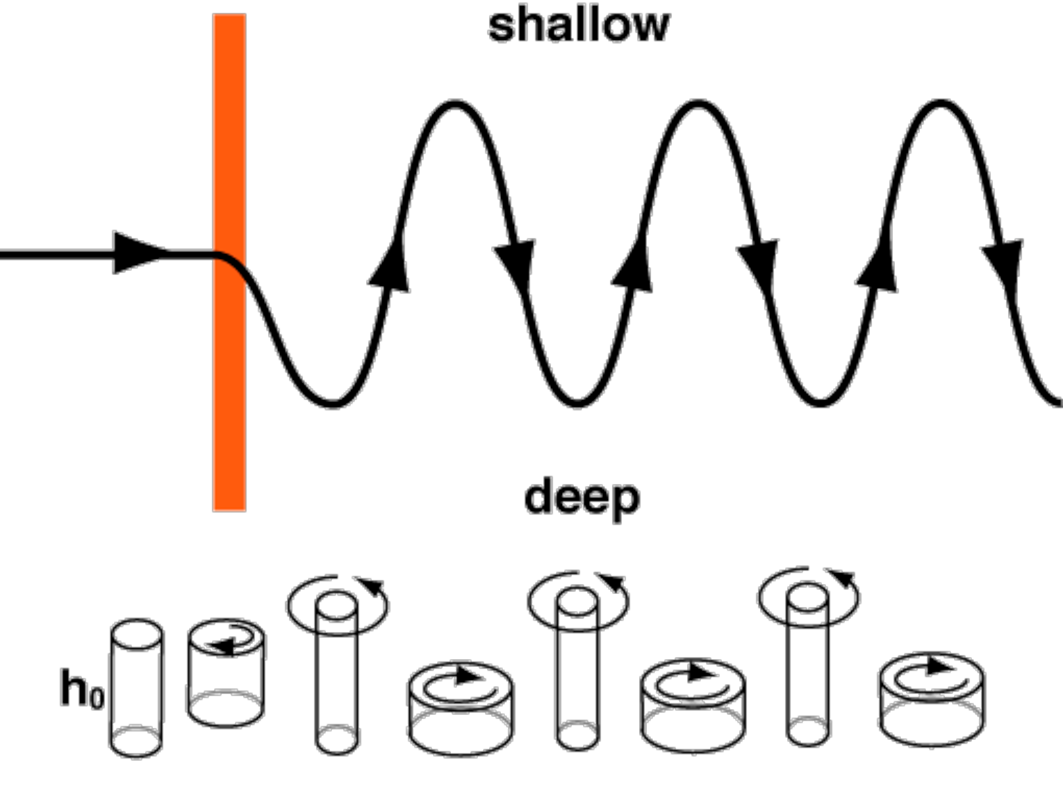
\includegraphics[width=0.65\hsize]{rossbyleewavesketch_cropped.pdf}}
%
%Imagine eastward flow encountering a topographic ridge.
%
%Sketch the evolution of the flow as it crosses the ridge and downstream of the ridge.
%
%
%%Rossby waves in eastward flow (Northern hemisphere), generated by
%%compression/stretching of vortex columns over the topography.   
%%North-South gradient of $f$ supports Rossby waves downstream.
%
%}
%






\end{document}







































